\documentclass[letterpaper,12pt]{article}
\usepackage{array}
\usepackage{threeparttable}
\usepackage{fancyhdr,lastpage}
\pagestyle{fancy}
\lhead{}
\chead{}
\rhead{}
\lfoot{}
\cfoot{}
\rfoot{\footnotesize\textsl{Page \thepage\ of \pageref{LastPage}}}
\renewcommand\headrulewidth{0pt}
\renewcommand\footrulewidth{0pt}
\usepackage[format=hang,font=normalsize,labelfont=bf]{caption}
\usepackage{listings}
\lstset{frame=single,
  language=Python,
  showstringspaces=false,
  columns=flexible,
  basicstyle={\small\ttfamily},
  numbers=none,
  breaklines=true,
  breakatwhitespace=true
  tabsize=3
}

\usepackage{geometry}
\geometry{letterpaper,tmargin=1in,bmargin=1in,lmargin=1in,rmargin=1in}
%\renewcommand\headrulewidth{2pt}
%\renewcommand\footrulewidth{2pt}
\usepackage{amsmath}
\usepackage{amssymb}
\usepackage{amsthm}
\usepackage{mathtools}
\usepackage{pdflscape}
\usepackage{harvard}
\usepackage{setspace}
\usepackage{float,color}
%\usepackage{enumitem}
\usepackage[pdftex]{graphicx}
\usepackage{hyperref}
\hypersetup{colorlinks,linkcolor=red,urlcolor=blue}
\theoremstyle{definition}
\newtheorem{theorem}{Theorem}
\newtheorem{acknowledgement}[theorem]{Acknowledgement}
\newtheorem{algorithm}[theorem]{Algorithm}
\newtheorem{axiom}[theorem]{Axiom}
\newtheorem{case}[theorem]{Case}
\newtheorem{claim}[theorem]{Claim}
\newtheorem{conclusion}[theorem]{Conclusion}
\newtheorem{condition}[theorem]{Condition}
\newtheorem{conjecture}[theorem]{Conjecture}
\newtheorem{corollary}[theorem]{Corollary}
\newtheorem{criterion}[theorem]{Criterion}
\newtheorem{definition}[theorem]{Definition}
\newtheorem{derivation}{Derivation} % Number derivations on their own
\newtheorem{example}[theorem]{Example}
\newtheorem{exercise}[theorem]{Exercise}
\newtheorem{lemma}[theorem]{Lemma}
\newtheorem{notation}[theorem]{Notation}
\newtheorem{problem}[theorem]{Problem}
\newtheorem{proposition}{Proposition} % Number propositions on their own
\newtheorem{remark}[theorem]{Remark}
\newtheorem{solution}[theorem]{Solution}
\newtheorem{summary}[theorem]{Summary}
\numberwithin{equation}{section}
\bibliographystyle{aer}
\newcommand\ve{\varepsilon}
\newcommand\boldline{\arrayrulewidth{1pt}\hline}
\newcommand{\q}[1]{``#1''}

\def\changemargin#1#2{\list{}{\rightmargin#2\leftmargin#1}\item[]}
\let\endchangemargin=\endlist 

\usepackage{graphicx}
\graphicspath{ {images/} }

\usepackage{enumerate}
%\usepackage[shortlabels]{enumerate}
\setlength{\parindent}{24pt}
%\renewcommand{\baselinestretch}{2.0}
\usepackage{lipsum} % just for the example
\makeatletter
\newcommand{\verbatimfont}[1]{\renewcommand{\verbatim@font}{\ttfamily#1}}
\makeatother
%\usepackage{enumitem}
\usepackage{float}

\verbatimfont{\small}%


\begin{document}

\begin{flushleft}
   \textbf{\Large{Problem Set \#2}} \\
   MACSS 30100 \\
   Luxi Han, 10449918\\
\end{flushleft}

\noindent \textbf{\large Problem 1}\par

\begin{enumerate} [\bfseries (a)]
\item The following graph is the histogram for the income of the MACSS cohort:\\
	\begin{figure}[H]
    		\centering
		\fbox{\resizebox{4.75in}{3in}{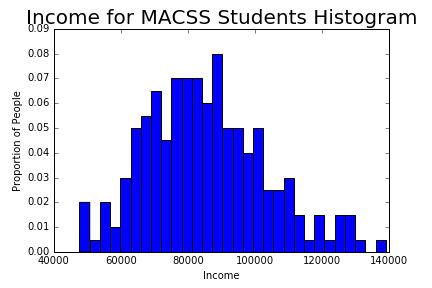
\includegraphics{hist_income}}}\
    		\caption{Histogram of Income of MACSS Students}
	\end{figure}\par
	
\item The value of the log likelihood value is -15829.239. The log normal pdf is as following.\par
	\begin{figure}[H]
    		\centering
		\fbox{\resizebox{4.75in}{3in}{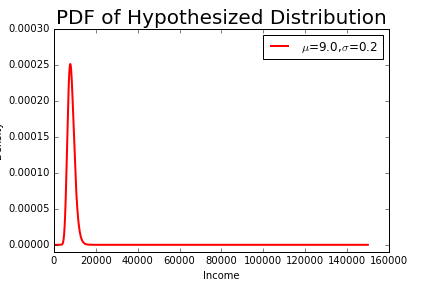
\includegraphics{hypo_pdf}}}\
    		\caption{Hypothesized PDF Distribution}
	\end{figure}\par

\item After the MLE estimation we have: \(\mu_{MLE} = 11.33; \sigma_{MLE} = 0.21 \). The value of the log likelihood function is -2239.53; the variance and covariance matrix is following:\\
\[
\begin{bmatrix}
2.18801e-04 &  6.47943e-06\\
6.47943e-06  & 1.19570e-04\\
\end{bmatrix}
\]
The following is the approximate value:\\
\[
\begin{bmatrix}
 0.00022&  0.00001\\
 0.00001&  0.00012\\
\end{bmatrix}
\]
The plotted graph is as following:\\
	\begin{figure}[H]
    		\centering
		\fbox{\resizebox{5in}{3in}{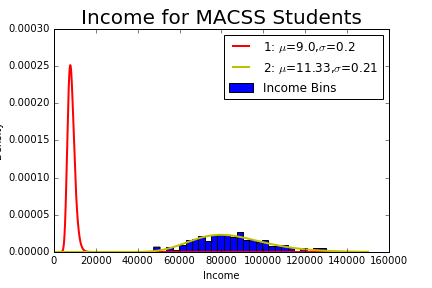
\includegraphics{dist_income}}}\
    		\caption{Distribution of Income}
	\end{figure}\par

\item  We have H0: \(\mu = 9.0\) and \(\sigma = 0.3\);\\
Chi squared of H0 with 2 degrees of freedom p-value =  0.0\\
We should reject the null hypothesis\par

\item We have the following result:\\
\begin{verbatim}
		The possibility of having an income higher than $100000 is 0.196
		The possibility of having an income lower than $75000 is 0.308
\end{verbatim}

\end{enumerate}

\noindent \textbf{\large Problem 2}\par

\begin{enumerate} [\bfseries (a)]
\item The following is the estimate:
\begin{align*}
\sigma_{MLE} &= 0.00302\\
\beta_0 &= 0.25164\\
\beta_1 &= 0.01293\\
\beta_2 &= 0.40050\\
\beta_3 &= -0.00999
\end{align*}
The log likelihood function value is \(876.86\).\\
The variance and covariance matrix is:\\
\[
\begin{bmatrix}

 1.&  0.&  0.&  0.&  0.\\
 0.&  1.&  0.&  0. & 0.\\
 0.&  0.&  1.&  0.&  0.\\
 0.&  0.&  0.&  1.&  0.\\
 0.&  0.&  0.&  0.&  1.\\
\end{bmatrix}
\]
\item
The null hypothesis:\\
\(H_0: \sigma^2 = 0.01, \beta_1, \beta_2, \beta_3, \beta_0 = 0\)\\
The p-value for the null hypothesis is approximately 0.00. We should reject the null hypothesis.

\end{enumerate}

\end{document}